\documentclass[a4paper,11pt,twoside]{book}

\usepackage{ifareport}

\usepackage{booktabs}
\usepackage{rotating}
\usepackage{array}
\usepackage{algorithmicx}
\usepackage{algorithm}
\usepackage{algpseudocode}
\usepackage{amsmath}
\usepackage{bm}


\setlength{\parskip}{1em}

%% EE Commands
\newcommand\ezz[1]{{\color{blue}#1}}

%% Configuration %%%%%%%%%%%%%%%%
\title{Karma Mechanisms for Congestion Management}
\author{Angel Manzano}
\thesistype{Semester Project}
\date{\today}
\advisors{Dr. Carlo Cenedese, Ezzat Elokda}
\keywords{advanced, quantum, psychology}

%% hyperref configuration %%%%%%%%%%%%%%%%%%%%%%%%%%%%
\loadhyperref

\let\oldcite\cite
\renewcommand*\cite[1]{{[\oldcite{#1}]}}

\begin{document}

\hyphenation{}

%% Cover %%%%%%%%%%%%%%%%%%%%%%%%%%%%%%%%%%%%%%%%%%%%%%%%%%%%%%%%%%%
\maketitle



%% List of contents %%%%%%%%%%%%%%%%%%%%%%%%%%%%%%%%%%%%%%%%%%%%%%%%%%%%%%
\cleardoublepage
\tableofcontents
\cleardoublepage
\addcontentsline{toc}{chapter}{List of Figures}
\listoffigures
\cleardoublepage
\addcontentsline{toc}{chapter}{List of Tables}
\listoftables					
\cleardoublepage
\mainmatter


%% Chapter %%%%%%%%%%%%%%%%%%%%%%%%%%%%%%%%%%%%%%%%%%%%%%%
\chapter{Introduction}

\textcolor{blue}{Introduce project: problem to be solved (a more fair and less monetary-based approach to congestion management) and the idea for the solution (implement Karma mechanism as the model for resource allocation).}

%% Section %%%%%%%%%%%%%%%%%%%%%%%%%%%%%%%%%%%%%%%%%%%%%%%
\section{Literature review- Karma Mechanism and Congestion Management}

\textcolor{blue}{In this section, talk about the Karma game paper by Ezzat, and link the main ideas to congestion management. Also review some of the most relevant congestion management papers.}

% This project is a continuation of the work done in AAAAA \ignore{Insert Ezzat's paper on karma}. In this chapter, the resource allocation mechanism will be formally presented, defining the most important parameters and their mathematical implementation. Since the desired use of the mechanism is that of control of road congestion, some relevant Congestion Management papers will also be explored, which will allow for the implementation of the Karma mechanism into a congestion model.


%% Subsection %%%%%%%%%%%%%%%%%%%%%%%%%%%%%%%%%%%%%%%%%%%%%%%
\subsection{Karma Mechanism review}


%% Subsection %%%%%%%%%%%%%%%%%%%%%%%%%%%%%%%%%%%%%%%%%%%%%%%
\subsection{Congestion Management models review}

As mentioned, this project looks to implement the Karma resource allocation mechanism in a model for vehicle congestion in a bottleneck. For this, some relevant tradable driving licenses models used for congestion management were studied, in order to grasp a deeper understanding of the problem to solve and the type of model that can be designed to work with the Karma mechanism.

To explain a simple bottleneck congestion model, let us refer to \cite{Xiaoetal}. This paper explains very clearly how the accumulative arrivals to the bottleneck and the queuing time for each arrival time evolve throughout the rush hour period.

The paper starts by differentiating between the types of costs that the drivers may experience when encountering a bottleneck: the queuing delay cost and the schedule delay penalty. The queuing delay cost is defined as the cost that the driver faces due to being stuck in traffic, while the schedule delay penalty defines the cost the driver induces due to not arriving at their destination (usually assumed to be the place of work) at the desired time, but rather being early or late. In most studies conducted up until now, these costs are directly related to the value of time (VOT) of each driver, which in turn is proportional to the monetary value of their time. This means that a driver whose time can be valued higher will incur a greater cost than a driver with a lower VOT. Since, at the equilibrium of the system, every player suffers the same cost, this means drivers with lower VOT will have to suffer either greater queuing or schedule delays, which might not be fair for them. This problem is solved by the use of the Karma mechanism, since the VOT of the divers cannot be measured by their monetary value, but rather by their urgency levels, and one cannot have the same level of urgency every day, because then they will run out of their karma ``points,'' and not be able to play the game.

The evolution of the queue is quite logical: the road has a limited capacity, so if at a single instant more cars arrive at the entrance of the bottleneck than the road is able to fit, traffic will start building up. If the desired work time is the same for all drivers, and the total number of drivers is greater than the total capacity of the road over the rush period, a queue will start forming, and growing as more drivers arrive. Therefore, the queuing time will increase proportionally to the queue building up. On the other hand, if the driver arrives earlier to the bottleneck, the queue they will experience is shorter, but their schedule delay will be greater, since they will arrive earlier at work than at their desired time.

The model can be made more complex, introducing time-varying credit charging or nonidentical commuters.

The article \cite{Verhoef} presents the cost function for a driver in a bottleneck model that is often used for congestion management models with tradable licenses:
\begin{equation}
    p(t) = \alpha T_q(t) + \beta \cdot max\{0, t^*-t-T_q(t)\} + \gamma \cdot max\{0, t+T_q(t)-t^*\} + \tau(t')
\end{equation}

Where $p(t)$ is the cost, $\alpha$ the VOT of the driver, $T_q(t)$ the queue time, $\beta$ and $\gamma$ the unit schedule early and late costs, respectively, $t'$ the exit time of the bottleneck, $\tau(t')$ a road toll as a function of the exit time, and $t^*$ the desired arrival time. 

Depending on the model, the function may have different parameters and variables.

The model including the Karma mechanism can be designed based on this cost function, with a few modifications:
\begin{enumerate}
    \item The multipliers cannot be based on the VOT or monetary value of the time of the commuters. Instead, as a multiplier it may make sense to use the urgency level of the agent, so the greater the urgency the greater the cost incurred, so the driver will try to minimize its queue and schedule delay penalties. It can do that by bidding a greater amount of karma, which, as will be explained later, will allow the agent to enter a faster lane and avoid any type of queue.
    
    \item The cost will depend on which type of lane the agent uses, as it may enter a faster lane with no queue, or a slow lane in which traffic may be built up, depending on the number of drivers that want to enter.
    
    \item The road toll may or may not be implemented, depending on the objective of the designer.
\end{enumerate}

The cost function used for the Karma mechanism will be presented in section 2.1.4.

%% Section %%%%%%%%%%%%%%%%%%%%%%%%%%%%%%%%%%%%%%%%%%%%%%%
\section{Organization of the paper}

This paper is structured as follow: the Karma resource allocation mechanism and some of the most important features of congestion management model for a bottleneck are introduced, in order to get perspective of the problem to be tackled, which is the implementation of a ``karma game'' for vehicle traffic control. In the second chapter, this implementation will be developed, first by defining the main parameters that the karma dynamic population game for this case is based on, and then by presenting the steps followed to reach the equilibrium of the game. Next, a case-study is investigated, with certain set-up values for, for example the possible urgency levels of the agents. The last chapter of the paper discussed the work done, the results obtained, and future works to be done to improve and expand the model.

\textcolor{blue}{Structure of the paper.}

%% Chapter %%%%%%%%%%%%%%%%%%%%%%%%%%%%%%%%%%%%%%%%%%%%%%%
\chapter{Implementing the Karma Mechanism into a Congestion Management model}

\textcolor{blue}{Explain how to introduce the Karma game into existing congestion management models. Present the Karma mechanism as a dynamic population game, defining the main components. Next, present the algorithm followed to find the SE and the variables needed to reach it.}


In this chapter, a new congestion management model will be presented, which implements the Karma mechanism for resource allocation. In the case of a simple bottleneck, this resource will be defined as the possible lanes the agents can take to get from the starting point of the bottleneck to the desired destination, as seen in the simple O-D sketch below.

The bottleneck model that will be used is a simple model with two different lanes: a fast lane without congestion, and a slow lane which could potentially have built up traffic.

\begin{figure}[h]
     \centering
     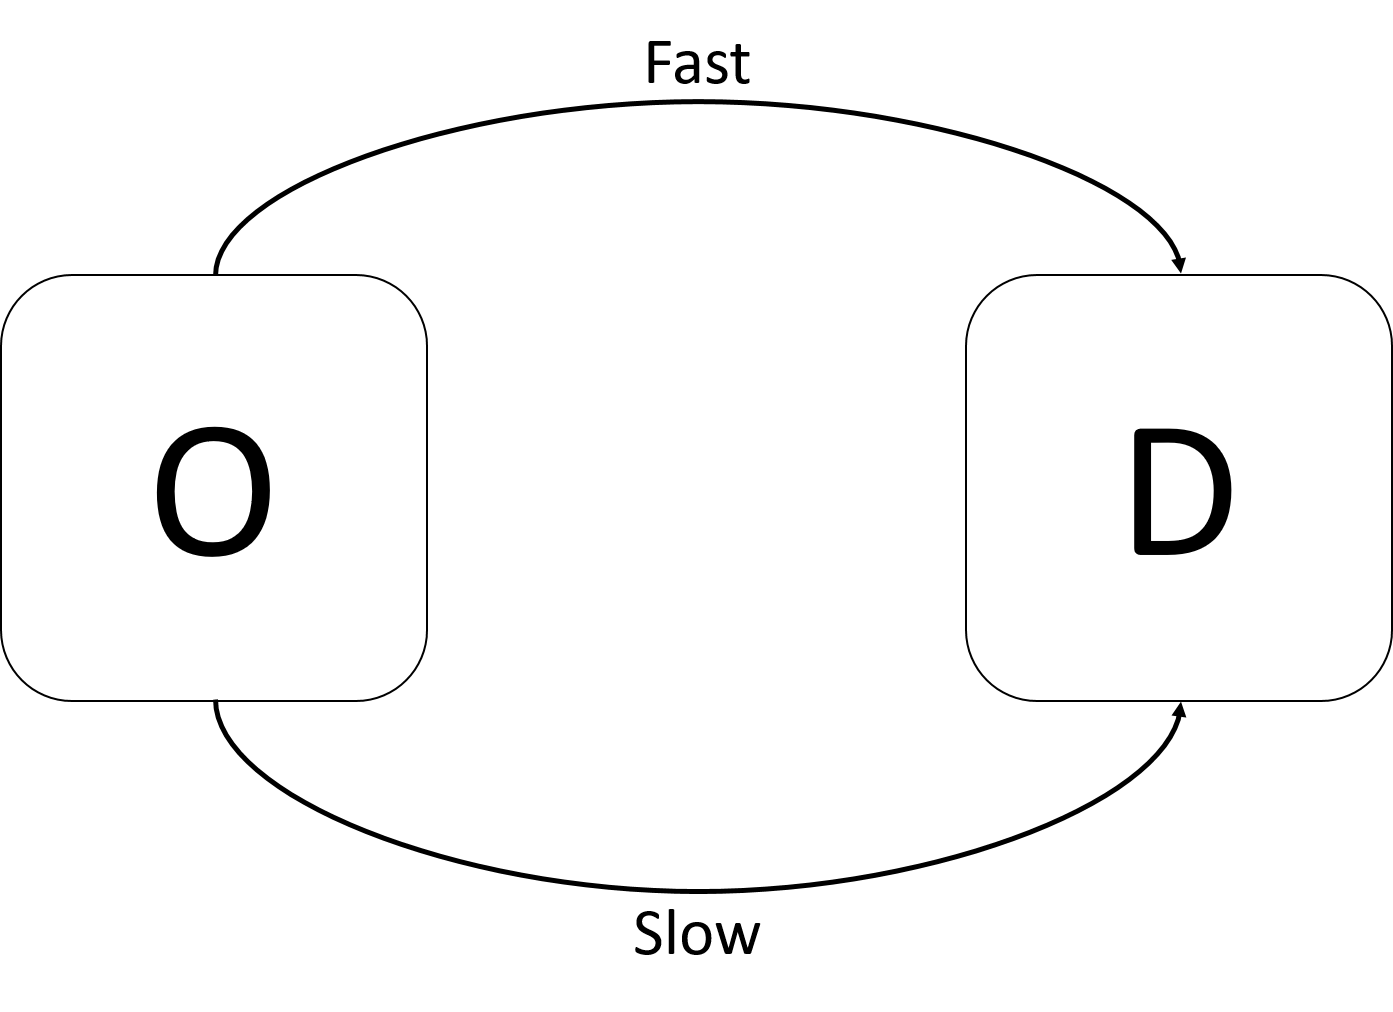
\includegraphics[width=0.6\textwidth]{reporttemplate/graphics/OD-pic2.png}\\
     \caption{O-D sketch}\label{fig:od_sketch}
\end{figure}

This chapter is divided into two parts: definition of the dynamic population game used to find the stationary equilibrium of the model, and the mathematical formulation of the most important variables for the Stationary Solution of the game.


%% Section %%%%%%%%%%%%%%%%%%%%%%%%%%%%%%%%%%%%%%%%%%%%%%%
\section{Dynamic population game definition}

As previously mentioned, the mechanism used is a continuation of the Karma mechanism for resource allocation. This mechanism is based on a dynamic population game (refer to \cite{DynPopGame} for an in-depth explanation of this type of games), more specifically on the formulation followed in \cite{KarmaGame}. 

One of the main differences between the game followed in the original Karma mechanism paper and the one followed here is the introduction of the time parameter inherent to vehicle bottleneck management. As was explained in section 2.2, for a bottleneck model, the agents can be defined by the time the arrive at the ``entrance'' of the bottleneck. This time variable is not present in the original Karma game, so it must be introduced as a new parameter of the game. More properly speaking, this new time parameter, called \textit{arrival time}, defines the type of the agents.

Thus, the Karma game for congestion management can be defined as following:

%% Subsection %%%%%%%%%%%%%%%%%%%%%%%%%%%%%%%%%%%%%%%%%%%%%%%
\subsection{Agent population}

The number of agents N is large enough such that the population can be considered a continuum of mass. Each agent $i$ can be defined by their arrival time, $t^i$, at the bottleneck, and their future awareness, $\alpha^i$. These two values describe the type $\tau$ of each agent, which can be formulated as follow:
\begin{equation*}
    \tau^i \in \mathcal{T}^i = (t^i, \alpha^i) \qquad \forall i = 1, ..., N
\end{equation*}

For simplicity, let us assume the arrival time $t^i$ of each agent is independent of the day, i.e. they will always reach the bottleneck at the same time instant every day.

Since each agent only plays the resource game once per day, at the moment of their arrival to the bottleneck, their actions can be modeled by a discrete-time Markov chain.

For the remainder of the paper, let us drop the superscript $i$ and assume every agent has the same defining parameters.


%% Subsection %%%%%%%%%%%%%%%%%%%%%%%%%%%%%%%%%%%%%%%%%%%%%%%
\subsection{Agent states}

As in \cite{KarmaGame}, each agent has a private state $x$, which is made up of their urgency level, $u$, and their karma level, $k$:
\begin{gather*}
    x = (u, k) \in \mathcal{X} = \mathcal{U} \times \mathcal{N} \\
    u \in \mathcal{U} = \{u_1, ..., u_{n_u}\} \\
    k \in \mathcal{N}
\end{gather*}

The urgency $u$, as its name indicates, is a representation of the importance of the desired resource to the agents. At consecutive time instants, which in this congestion management framework means at the same arrival time but in consecutive days, the urgency levels of the agents follow an exogenous, irreducible Markov chain process. The probabilities of progressing from one urgency value to the next are denoted by:
\begin{equation*}
    \phi [u^+ \mid u]
\end{equation*}

Let us assume the urgency levels of the agents are independent from each other, and that the process for all agents follow the same transition probabilities. An explanation for this assumption is given in \cite{KarmaGame}.


%% Subsection %%%%%%%%%%%%%%%%%%%%%%%%%%%%%%%%%%%%%%%%%%%%%%%
\subsection{Social state}

The state of the whole population at a given time is composed of two parameters: the distribution of the agents' states and the bid policy.

The distribution of agents' states is defined as:
\begin{equation*}
    d\in \mathcal{D} = \Delta(\mathcal{X}) = \left\{d \in \mathbb{R}_+^{\infty} \bigm\vert \sum_{u,k} d[u,k,t] = 1 \right\}
\end{equation*}

$d[u,k,t]$ represents the fraction of agents at the state $(u,k)$ at any time instant $t$. 

The action of any agent is defined by the bid they decide to play at their arrival time, delimited by their karma level and zero, i.e. an agent cannot bid less than zero or more than the karma they currently have. 
\begin{equation*}
    b \in \mathcal{B}^k = \{b \in \mathbb{N} \mid 0 \leq b \leq k\}
\end{equation*}

Therefore, the homogeneous policy they follow is:
\begin{equation*}
    \pi \in \Pi : \mathcal{X} \rightarrow \Delta(\mathcal{B}^k) = \left\{\sigma \in \mathbb{R}_+^{k+1} \bigm\vert \sum_{b} \sigma[b] = 1 \right\}
\end{equation*}

The policy maps the state of each agent to a probability distribution over the possible bids $b$. The probability of playing a certain bid given the current state of the agents is denoted by $\pi[b \mid u,k]$.

The pair $(d,\pi)$ is called the social state, and it follows a Markov decision process. When an equilibrium is reached, the defining parameters of the society have converged, i.e. the social state is stable. In order to define this Markov process, both an immediate reward function and a state transition function need to be defined. 


%% Subsection %%%%%%%%%%%%%%%%%%%%%%%%%%%%%%%%%%%%%%%%%%%%%%%
\subsection{Immediate reward function $\zeta[t,u,b](d,\pi)$}

In congestion management, the cost that is usually associated to the drivers when they encounter a bottleneck is defined by two values: the cost suffered from being stuck in the queue (Queuing Cost) and the cost from not arriving at the final destination at the desired time, either because the driver is too early or too late (Schedule Cost). Usually, these costs are multiplied by the value of time (VOT) of the driver. This VOT is inherently related to the monetary value of the time of the agents, which defeats the purpose of the Karma mechanism. For this reason, in this model, instead of the VOT the multiplier represents the urgency of the agents. It is clear to see that the more urgent an agent is, the higher the cost they will perceive if their waiting time or schedule delay is large.

Therefore, the immediate reward function is defined as:
\begin{equation}
    \begin{split}
        \zeta[u,b,t](d,\bm{\pi}) = u \Bigg[\gamma[o=0 \mid b,t](d,\bm{\pi}) \, (\psi |t^*-t|) \, + \\
        \, \gamma[o=1 \mid b,t](d,\bm{\pi}) \, (T_q[t](d,\pi) + \psi |t^*-t-T_q[t](d,\pi)|)\Bigg]
    \end{split}
\end{equation}

Where $\psi$ is the relation between the importance of the queuing cost to schedule cost, $t^*$ the desired exit time of the bottleneck, the function $\gamma$ defines the probability of obtaining a certain outcome given the bid of the agent and their bottleneck arrival time. In this case, more specifically the probability of winning the game at a given time (the meaning of this function will be explained later). Finally, $T_q$ is the queuing time in the slow lane (as previously mentioned, the fast lane accumulates no traffic). The whole expression is multiplied by the urgency value $u$, for the reason mentioned earlier.

In order to calculate the queuing time let us follow the following algorithm:

\begin{enumerate}
    \item Calculate number of agents that enter the slow lane at each time
    \begin{center}
        $n_s[t] = \sum_{b'} g[t] \cdot \gamma[o=1 \mid t,b']$
    \end{center}
    \item Calculate number of agents in the queue after arrival of new agents at each time 
    \begin{center}
        $q_s[t] = max(0, \, q_s[t-1] + n[t] - s_s + H[s])$
    \end{center}
    \item Calculate queuing time for agents arriving at each time 
    \begin{center}
        $T_q[t] = \frac{q_s[t]}{s_s}$
    \end{center}
\end{enumerate}

Where $s_s$ is the capacity of the slow lane, \(g[t] = \sum_{u',k'} d[u',k',t]\) is the fraction of total agents arriving at time $t$, and $H[t]$ the number of drivers that are not playing the karma game at time $t$, and thus enter the slow lane directly.

In order to obtain the function $\gamma$, it is first necessary to define the bid distribution of all agents:
\begin{equation}
    \nu[b'\mid t](d,\bm{\pi}) = \frac{\sum_{u',k'} d[u',k',t] \, \pi[b' \mid u',k',t]}{g[t]}\\
\end{equation}

The expression is divided by $g[t]$ in order to normalize the results, as is customary in population games.

This distribution can be represented by a histogram as follows:
\begin{figure}[H]
    \centering
    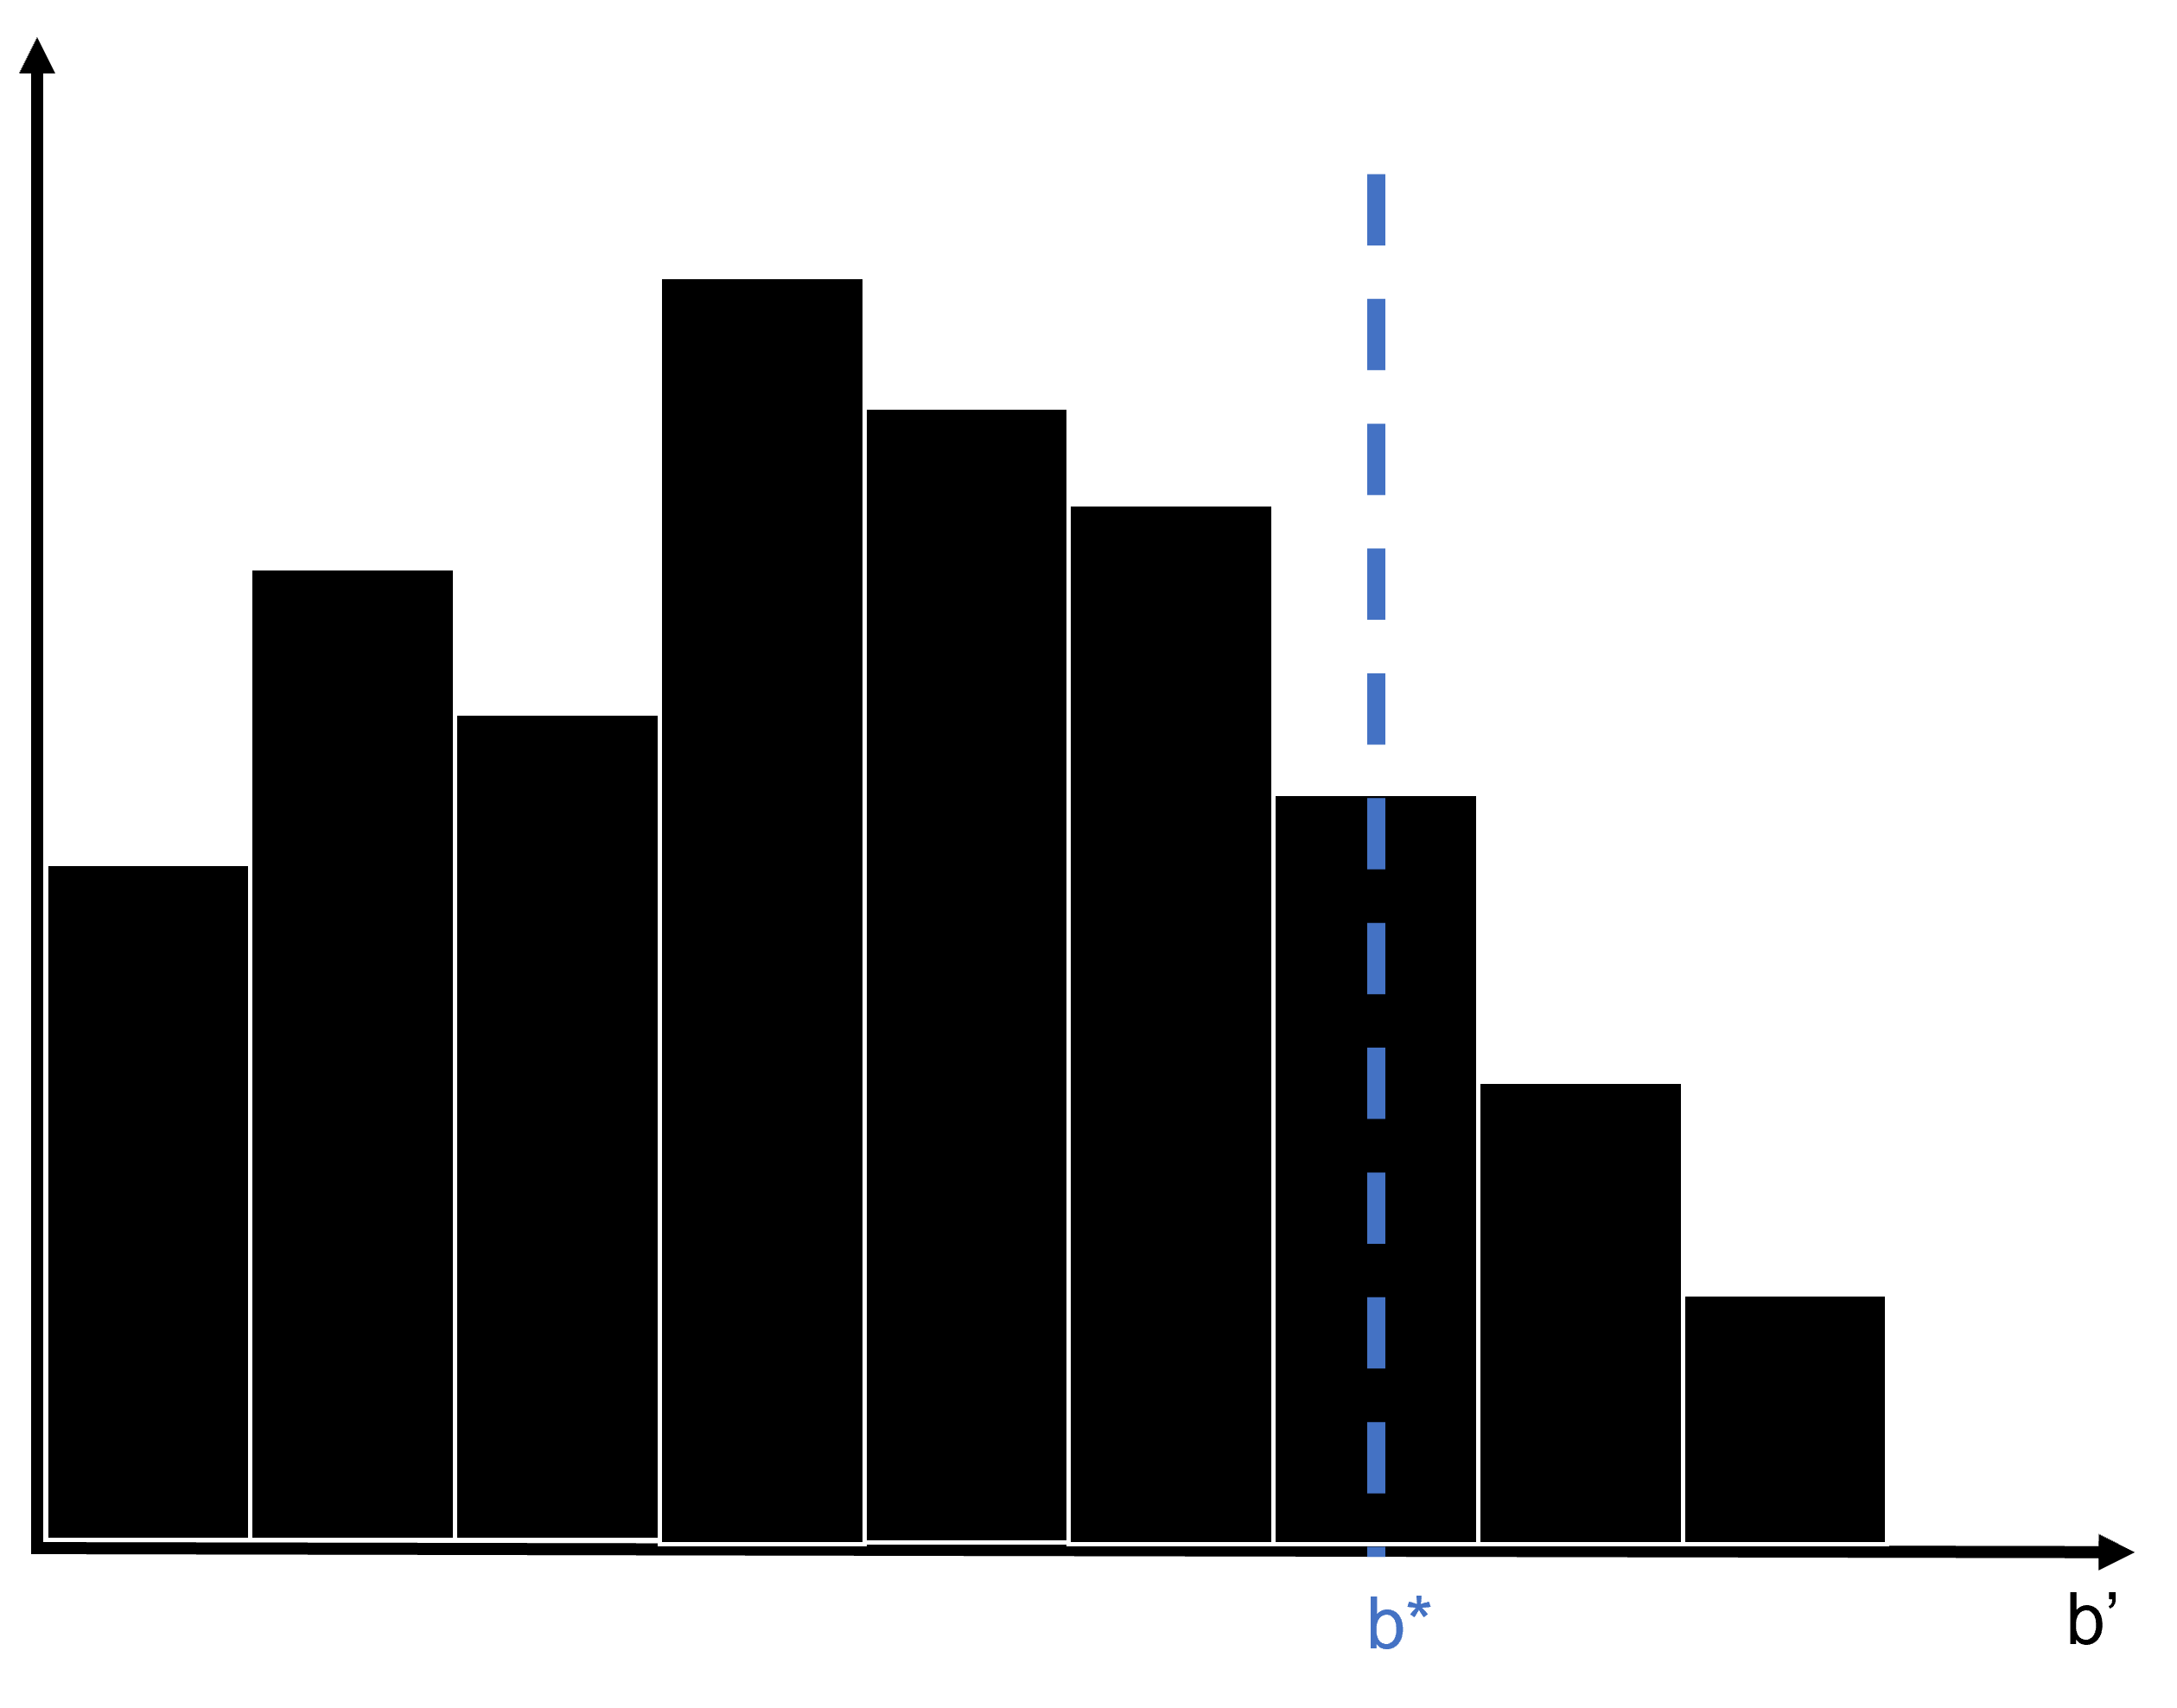
\includegraphics[width=0.5\textwidth]{reporttemplate/graphics/bid_distribution.png}\\
    \caption{Bid distribution of all agents- fake scenario}\label{fig:bid_distribution}
\end{figure}

$b^*$ can be interpreted as the maximum bid of agents who did not get in: those agents whose bids \textit{b} is $b<b^*$ have not won the game, and thus will have to go to the slow lane. On the other hand, those agents with bids such that $b>b^*$ are guaranteed to have won the bid and will be able to enter the fast lane. $b^*$ can be calculated as:
\begin{equation}
    \begin{array}{ll@{}ll}
        \text{max}  & b &\\
        \text{subject to}& \displaystyle\sum\limits_{b'>b}   &\nu[b'\mid t](d,\pi) + \nu[b\mid t](d,\pi) \geq \bar{s}
    \end{array}
\end{equation}

Where \(\bar{s} = \frac{s}{N} \Delta t\) is the fraction of vehicles that can enter the fast lane per time-step, \textit{s} is the capacity of the fast lane, and \textit{N} is the total number of agents who are playing the game.

The problem arises when the agents' bid is $b=b^*$. In this case, the outcome of the agents is determined probabilistically. In order to make the model simple, the probability of winning the bid is equal to the fraction of agents who decided to bid $b=b^*$ that can fill the capacity of the fast lane. The final outcome of the game for each player is formally defined through the function $\gamma[o \mid b,t](d,\bm{\pi})$.

$\gamma[o \mid b,t](d,\bm{\pi})$ can be defined as the probability of the game outcome of each agent (o=0 means the agents ``won'' the game, and o=1 the agent ``lost'' the game) depending on their bid and their arrival time. 

\begin{equation}
    \gamma[o = 0 \mid b,t](d,\bm{\pi}) = \begin{cases}
        1 & \text{if } (\nu[b \mid t] + \epsilon) + \sum_{b'<b} \nu[b' \mid t] \leq \bar{s} \\
        0 & \text{if } \sum_{b'>b} v[b' \mid t] \geq \bar{s} \\
        \frac{\bar{s} - \sum_{b'>b}\nu[b' \mid t]}{\nu[b \mid t] + \epsilon} & \text{if else}
    \end{cases}
\end{equation}

The value $\epsilon$ is introduced for numerical conditioning for the case in which $\nu[b \mid t] = 0$.

Consequently,  
\begin{center}
    $\gamma[o = 1 \mid b,t](d,\bm{\pi}) = 1 - \gamma[o = 0 \mid b,t](d,\bm{\pi})$
\end{center}







\newpage
%% Section %%%%%%%%%%%%%%%%%%%%%%%%%%%%%%%%%%%%%%%%%%%%%%%
\section{Dynamic population game formulation}

After some repetitions of the game, the agents will reach an equilibrium in their social state (d, $\pi$). This is called the \textit{Stationary Equilibrium}. The algorithm for finding this equilibrium is as follows:

\textbf{Input:} initial state distribution $d^0$ with average karma $\bar k$, initial policy $\pi ^0$, parameters $\eta, \gamma, dt$ 

\textbf{Initialize:} \textbf{b} $\leftarrow d^0$, $\bm{\pi} \leftarrow \pi^0$

\textbf{While ($\bm{d}, \bm{\pi}$)} do not converge:

\begin{enumerate}
    \item Compute:
    \begin{enumerate}
        \item $\nu[b',t](\bm{d},\bm{\pi})$, $\gamma[o \mid b,t](\bm{d},\bm{\pi})$, $\kappa[k^+ \mid k,b,o,t](d,\bm{\pi})$
        
        \item $\zeta[u,b,t](\bm{d},\bm{\pi})$, $\rho[u^+,k^+ \mid u,k,b,t](\bm{d},\bm{\pi})$
        
        \item $R[u,k,t](\bm{d},\bm{\pi})$, $P[u^+,k^+ \mid u,k,t](\bm{d},\bm{\pi})$
        
        \item $V[u,k,t](\bm{d},\bm{\pi})$, $Q[u,k,b,t](\bm{d},\bm{\pi})$
        
        \item $\bm{\tilde{\pi}}[b \mid u,k,t](\bm{d},\bm{\pi})$
    \end{enumerate}
    
    \item Forward-propagate the discretized evolutionary dynamics:
    \begin{gather}
        \bm{d} \leftarrow (1-dt) \, \bm{d} + dt \, \bm{d}P(\bm{d}, \bm{\pi})\\
        \bm{\pi}[\cdot \mid u,k] \leftarrow (1-\eta \, dt) \,  \bm{\pi}[\cdot \mid u,k] + \eta \, dt \, \tilde{\pi} [\cdot \mid u,k](\bm{d}, \bm{\pi})
    \end{gather}
\end{enumerate}


Next, the mathematical formulation of each variable present in the SE algorithm computation will be presented:

The bid distribution of all agents can be readily determined from the social state as follows:
\begin{equation}
    \nu[b'\mid t](d,\bm{\pi}) = \frac{\sum_{u',k'} d[u',k',t] \, \pi[b' \mid u',k',t]}{g[t]}\\
\end{equation}

Where \(g[t] = \sum_{u',k'} d[u',k',t]\) is the fraction of total agents arriving at time $t$. This is done in order to normalize the results, as is usually done in population games.\\

The bid distribution could be represented by a histogram as follows:

\begin{figure}[H]
    \centering
    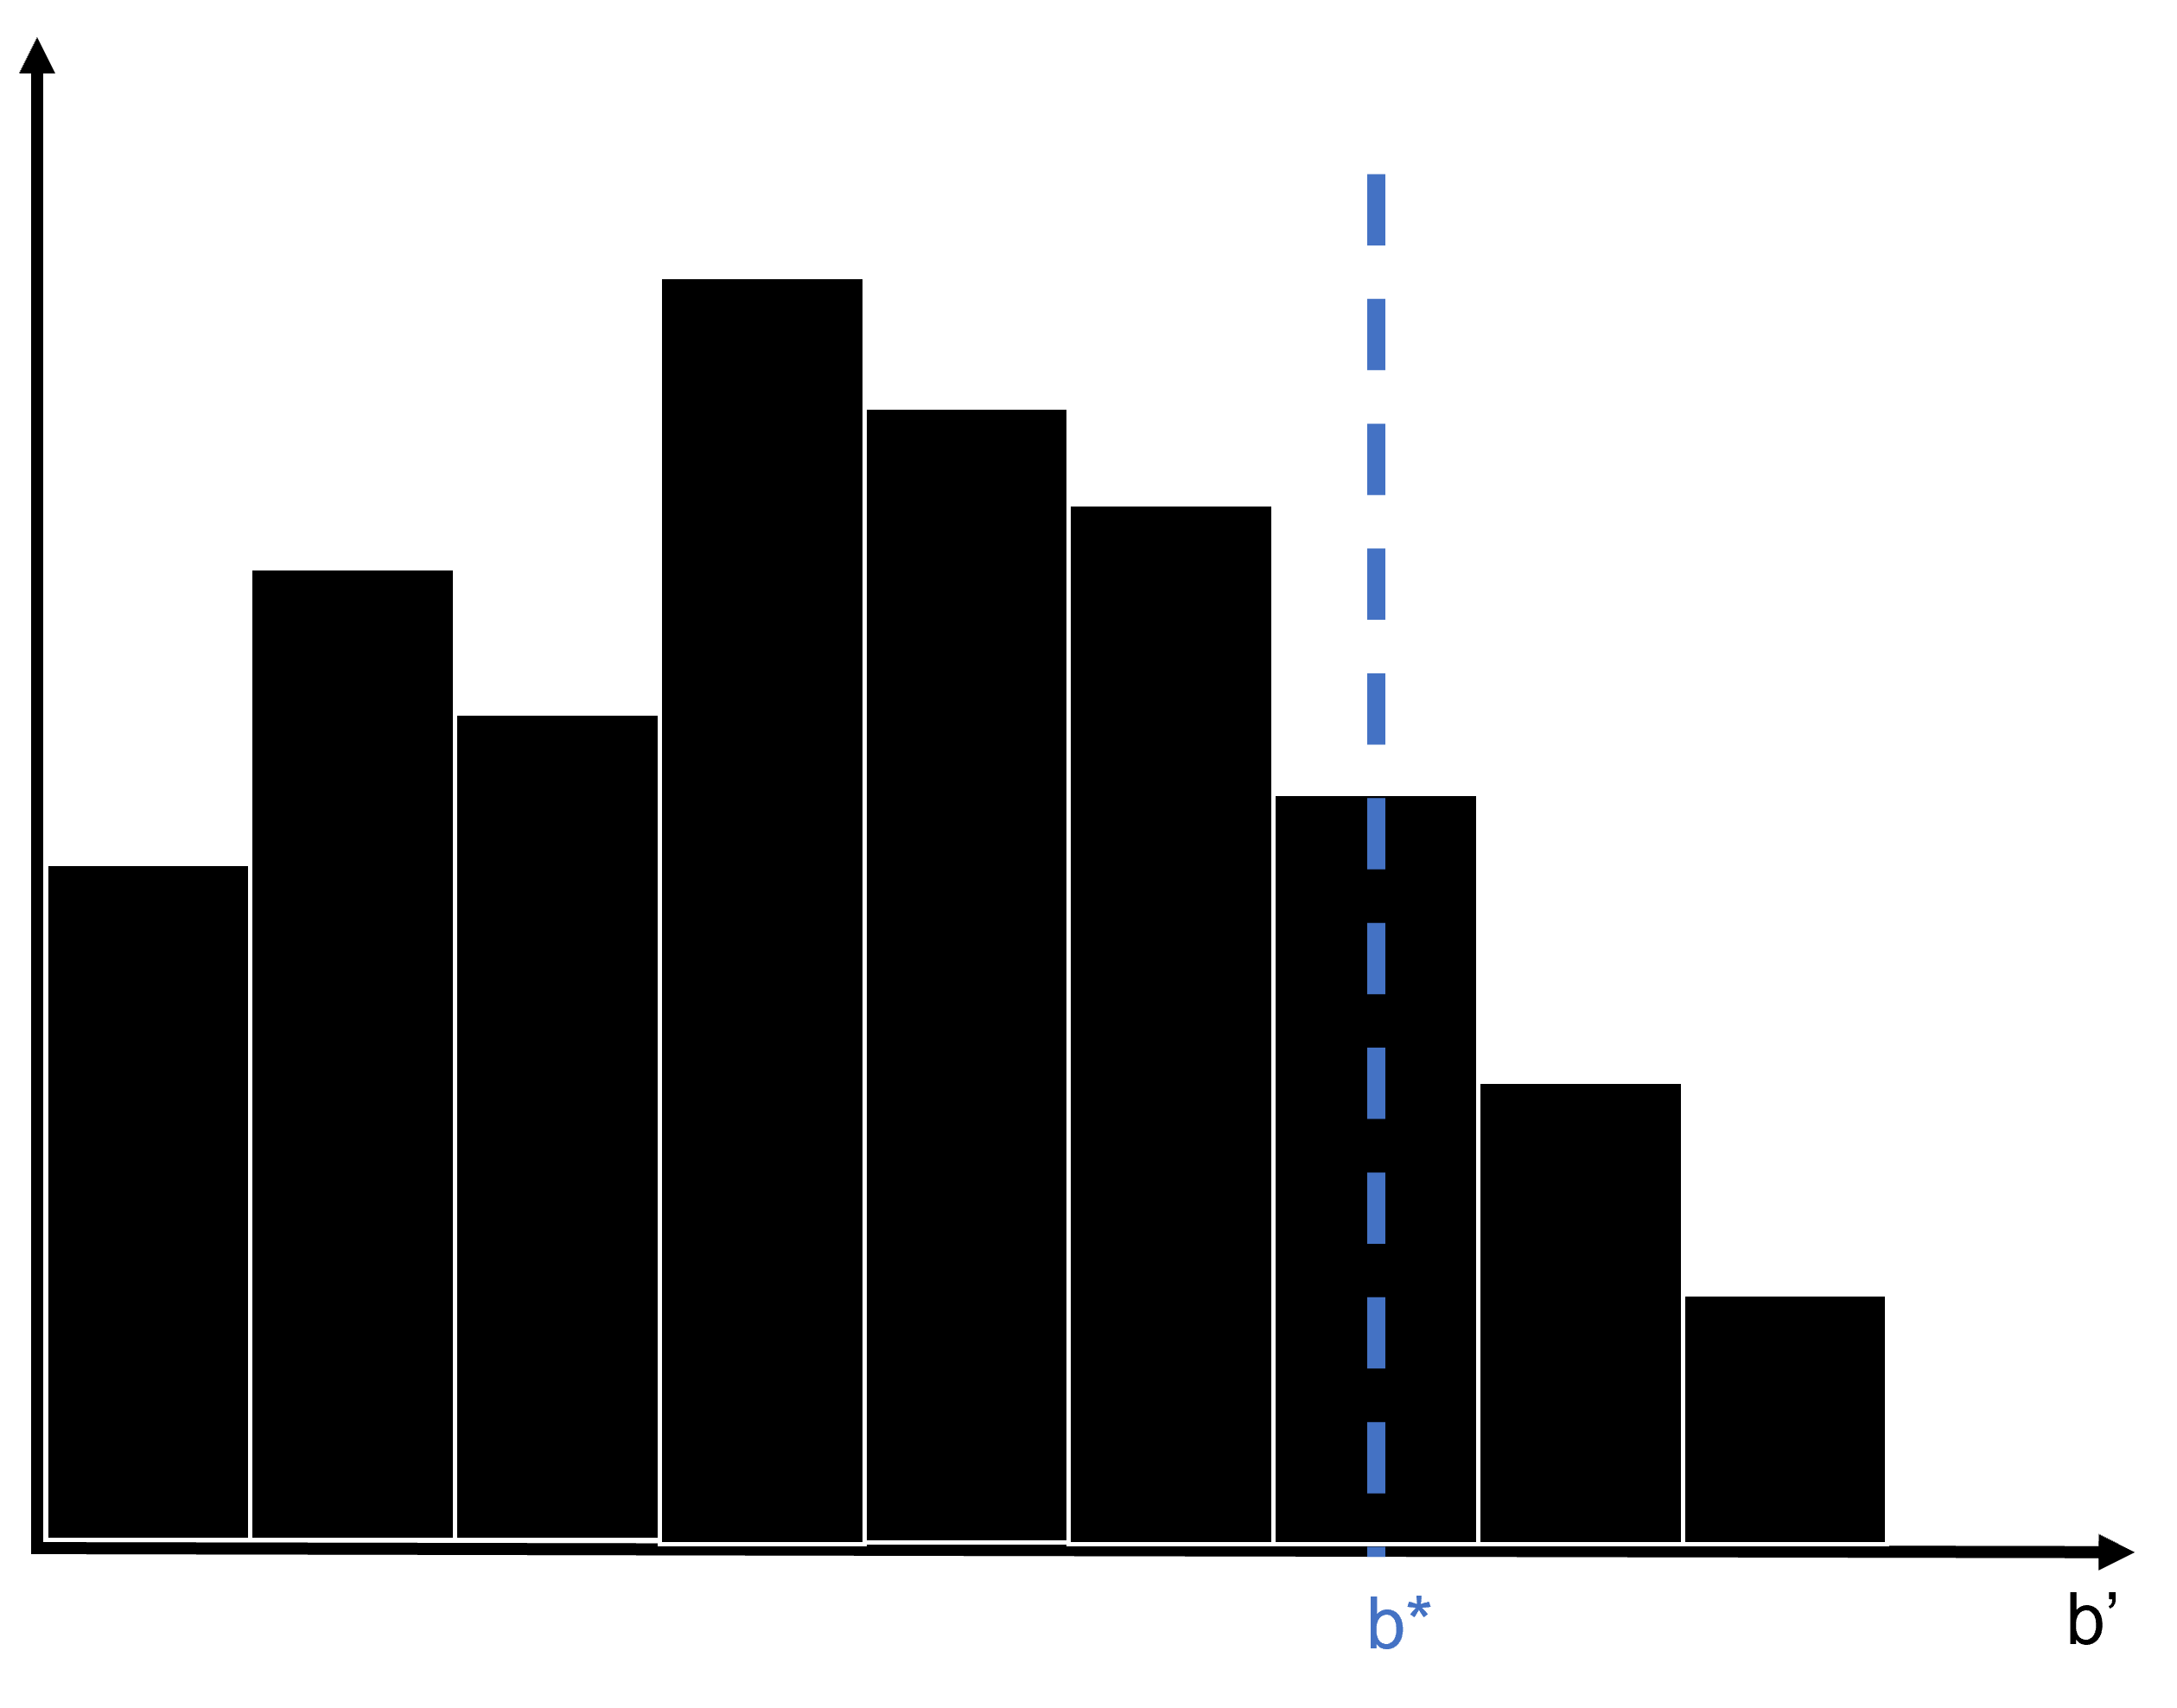
\includegraphics[width=0.6\textwidth]{reporttemplate/graphics/bid_distribution.png}\\
    \caption{Bid distribution of all agents}\label{fig:bid_distribution}
\end{figure}

$b^*$ can be interpreted as the maximum bid of agents who did not get in: those agents whose bids \textit{b} is $b<b^*$ have not won the game, ans thus will have to go to the slow lane. On the other hand, those agents with bids such that $b>b^*$ are guaranteed to have won the bid and will be able to enter the fast lane. $b^*$ can be calculated as:

\begin{equation}
    \begin{array}{ll@{}ll}
        \text{max}  & b &\\
        \text{subject to}& \displaystyle\sum\limits_{b'>b}   &\nu[b'\mid t](d,\pi) + \nu[b\mid t](d,\pi) \geq \bar{s}
    \end{array}
\end{equation}

Where \(\bar{s} = \frac{s}{N} \Delta t\) is the fraction of vehicles that can enter the fast lane per time-step, \textit{s} is the capacity of the fast lane, and \textit{N} is the total number of agents who are playing the game.

The problem arises when the agents' bid is $b=b^*$. In this case, the outcome of the agents is determined probabilistically. In order to make the model simple, the probability of winning the bid is equal to the fraction of agents who decided to bid $b=b^*$ that can fill the capacity of the fast lane. The final outcome of the game for each player is formally defined through the function $\gamma[o \mid b,t](d,\bm{\pi})$.

$\gamma[o \mid b,t](d,\bm{\pi})$ can be defined as the probability of the game outcome of each agent (o=0 means the agents ``won'' the game, and o=1 the agent ``lost'' the game) depending on their bid and their arrival time. 

\begin{equation}
    \gamma[o = 0 \mid b,t](d,\bm{\pi}) = \begin{cases}
        1 & \text{if } (\nu[b \mid t] + \epsilon) + \sum_{b'<b} \nu[b' \mid t] \leq \bar{s} \\
        0 & \text{if } \sum_{b'>b} v[b' \mid t] \geq \bar{s} \\
        \frac{\bar{s} - \sum_{b'>b}\nu[b' \mid t]}{\nu[b \mid t] + \epsilon} & \text{if else}
    \end{cases}
\end{equation}

The value $\epsilon$ is introduced for numerical conditioning for the case in which $\nu[b \mid t] = 0$.

Consequently,  $\gamma[o = 1 \mid b,t](d,\bm{\pi}) = 1 - \gamma[o = 0 \mid b,t](d,\bm{\pi})$.

As explained in the original karma paper, the karma transition function $\kappa[k^+ \mid k,b,o,t](d,\bm{\pi})$ is highly tunable, as long as the total karma in the system remains constant. One possible approach is the following:

Firstly, explained it words, the method followed for the redistribution of the karma is linearly dependent on the bid made by the agents, and only those agents who did not win the game (i.e. those with o=1) will be redistributed some karma.

It is possible to obtain the fraction, and total number, of agents that will enter the fast lane at each time-step, i.e. fraction and total number of agents with o=0:

\begin{gather}
    f_{o=0}[t] = \sum_{b'} \nu [b' \mid t](d,\pi) \cdot \gamma [o=0 \mid b',t](d,\pi)\\ 
    n_{o=0}[t] = \frac{N \cdot f_{o=0}[t]}{g[t]} 
\end{gather}





%% Chapter %%%%%%%%%%%%%%%%%%%%%%%%%%%%%%%%%%%%%%%%%%%%%%%
\chapter{Results}

\textcolor{blue}{Results of the simulation. Explanation of the results.}


%% Chapter %%%%%%%%%%%%%%%%%%%%%%%%%%%%%%%%%%%%%%%%%%%%%%%
\chapter{Conclusion}

\textcolor{blue}{Conclusion: review the main points of the paper and results obtained. Define future works}



\addcontentsline{toc}{chapter}{Bibliography}
\cleardoublepage
\printbibliography

\end{document}


%\begin{figure}
%     \centering
%     \includegraphics[width=.9\textwidth]{Wind_Turbine.jpg}\\
%     \caption{Romantic sunset with green power}\label{wind_turbine}
%\end{figure}

%\begin{figure}[H]
%    \ffigbox[\FBwidth] {
% 	\caption[Importes pedidos, pendientes, y entregados por año]{Importes pedidos, pendientes, y entregados por año}  
%    \label{fig:cantAño}
%    }
% 	{\includegraphics[scale=1]{Capitulo 3 imagenes/cantidadesAño.png}}
%\end{figure}


%% Bibliography %%%%%%%%%%%%%%%%%%%%%%%%%%%%%%%%%%%%%%%%%%%%%%%
%\addcontentsline{toc}{chapter}{Bibliography}
%\cleardoublepage
%\printbibliography